\documentclass[12pt]{article}
\usepackage[utf8]{inputenc}
\usepackage[T1]{fontenc}
\usepackage[french]{babel}
\usepackage{graphicx}
\usepackage{amsmath}
\usepackage{amssymb}
\usepackage{listings}
\usepackage{hyperref}
\usepackage{geometry}
\geometry{
  a4paper,
  total={170mm,257mm},
  left=20mm,
  top=20mm,
}

\title{Rapport du Projet : Moteur 3D}
\author{TRAORE \& YAMEOGO}
\date{2 janvier 2024}


\begin{document}

\maketitle
\begin{center}

\includegraphics[width=0.5\textwidth]{logo.png}
\end{center}

\vspace{5cm}

\noindent\textbf{Professeur Encadrant :} M. Vincent TORRI

\newpage
\tableofcontents
\newpage

\section{Introduction}
\label{sec:introduction}

\noindent Le rendu 3D, pierre angulaire de nombreux domaines tels que les jeux vidéo, l'architecture, la simulation et la conception assistée par ordinateur, consiste à générer des images bidimensionnelles à partir de modèles tridimensionnels. Ce processus implique une transformation des données géométriques, une gestion de la perspective, de la profondeur et de la visibilité, ainsi qu'un rendu visuel des objets qui respecte les contraintes visuelles de notre vision.  Parmi les techniques de rendu les plus utilisées, la rasterisation se distingue par sa capacité à offrir une performance élevée, la rendant incontournable pour des applications interactives en temps réel.

\noindent Ce rapport présente une analyse approfondie du développement d'un moteur 3D basique, réalisé dans le cadre du projet \textit{"Moteur 3D"} pour le cours de Programmation Avancée et Projet. Ce projet a été conçu comme une exploration pratique des mécanismes fondamentaux du rendu graphique 3D, en utilisant la bibliothèque SDL2. Notre objectif a consisté à élaborer une application capable de manipuler et d'afficher des objets 3D, tout en intégrant des mécanismes de contrôle interactif. Bien que modeste dans sa portée, ce moteur 3D nous a permis d'étudier en profondeur les défis associés au rendu par rasterisation, en nous confrontant aux problématiques de la programmation graphique. Ce rapport documente nos choix de conception, les difficultés techniques rencontrées, les solutions méthodologiques mises en œuvre, ainsi que les perspectives d'amélioration que nous envisageons.

\section{Choix de Conception}
\label{sec:choix_conception}

\noindent Dans cette section, nous allons détailler de manière approfondie les choix de conception qui ont guidé le développement de notre moteur 3D, en expliquant les raisons qui ont motivé chaque décision.

\subsection{Bibliothèque Graphique : SDL2}
\label{subsec:bibliotheque_graphique}

\noindent Nous avons opté pour la bibliothèque SDL2. SDL2 offre un bon compromis entre la gestion de bas niveau des ressources graphiques et les fonctions nécessaires pour la création de fenêtres et le rendu 2D. Son utilisation nous a permis de nous concentrer sur les aspects fondamentaux du rendu 3D sans nous perdre dans les détails spécifiques des API d'affichage du système d'exploitation. De plus, étant donné que ce cours était basé sur l'utilisation de SDL2, c'était un choix pertinent pour notre projet.

\subsection{Modélisation des Objets 3D}
\label{subsec:modelisation_objets}

\noindent Pour la représentation des objets 3D, nous avons choisi une approche par facettes, en décomposant les objets en surfaces planes (les polygones) :
\begin{itemize}
    \item \textbf{Point3D} : Représente un point dans l'espace 3D, défini par trois coordonnées flottantes $x$, $y$, et $z$. Le choix du type \textit{float} assure une plus grande précision et évite des erreurs de calcul lors des transformations géométriques. Nous avons encapsulé ces trois coordonnées dans une classe nommée \texttt{Point3D} pour plus de clarté.
    \item \textbf{Triangle3D} : Représente un triangle dans l'espace 3D, défini par trois objets \textit{Point3D} qui représentent ses sommets. Cette classe permet la manipulation des triangles et facilite la construction d'objets 3D. 
    \item \textbf{Quad3D} : Représente un quadrilatère 3D, défini par quatre objets \textit{Point3D}. Cette classe a été créée dans le but de faciliter la construction d'objets comme le cube, qui est naturellement constitué de quadrilatères. Cette classe est celle que nous allons utiliser par la suite pour tous nos rendus.
    \item \textbf{Scene3D} : Permet de gérer l'ensemble de la scène 3D, en contenant une collection d'objets \textit{Quad3D}. Cette approche permet de structurer le code et d'avoir une vue d'ensemble des objets qui composent la scène.
\end{itemize}

\noindent Ce choix nous a permis de nous familiariser avec la technique du rendu par rasterisation, utilisée dans la plupart des cartes graphiques modernes. De plus, nous avons choisi d'utiliser la technique du "triangle fan" pour le rendu et le remplissage des quadrilatères. Cela nous a permis de simplifier le rendu en décomposant un quadrilatère en deux triangles lors de l'affichage, sans que cela ne nécessite d'ajouter des méthodes supplémentaires.

\subsection{Classes de Base pour le Rendu et la Projection}
\label{subsec:classes_base}

\noindent En plus des classes dédiées à la modélisation 3D, notre projet inclut les classes suivantes, essentielles pour le rendu :
\begin{itemize}
  \item \textbf{Point2D} : Représente un point dans l'espace 2D de l'écran. Elle contient les coordonnées entières x et y nécessaires pour les fonctions de dessin de SDL. Les coordonnées de la classe \textit{Point3D} sont converties en coordonnées \textit{Point2D} grâce à la projection, et ces coordonnées sont utilisées lors du rendu des polygones.
  \item \textbf{Sdl} : Cette classe encapsule toutes les fonctionnalités de SDL, permettant une gestion plus structurée de l'initialisation, de la création de la fenêtre et du moteur de rendu, ainsi que leur libération. Cela a amélioré notre organisation du code et a garanti une libération correcte des ressources SDL. Elle fournit des méthodes pour la gestion de la fenêtre, de la surface d'affichage, et pour l'utilisation du moteur de rendu. Cette approche permet de ne pas polluer le main avec la gestion des ressources SDL et permet une approche beaucoup plus propre.
\end{itemize}

\label{sec:diagramme}

\noindent Le diagramme UML qui résume l'architecture de notre projet est présenté \textit{figure \ref{fig:uml}}. Ce diagramme a été réalisé avec draw.io.

\begin{figure}[h]
\begin{center}
\includegraphics[width=1.0\textwidth]{uml.jpg}
\end{center}
\caption{Diagramme UML du projet}
\label{fig:uml}
\end{figure}

\subsection{Fonctions de Transformation et de Rendu}
\label{subsec:fonctions_transformations}

\noindent Plusieurs fonctions clés ont été développées pour gérer les transformations, le rendu et la manipulation des objets 3D :
\begin{itemize}
    \item \textbf{rotatePoint} : Cette fonction prend un point 3D en entrée et applique une transformation de rotation autour des axes X et Y. Elle utilise les matrices de rotation pour transformer la position du point de manière correcte, et est la base des rotations appliquées aux objets de la scène. Cette fonction utilise un système de coordonnées cartésiennes.
    \item \textbf{project} : Cette fonction effectue la projection d'un point 3D sur le plan 2D de l'écran, en utilisant un facteur d'échelle basé sur la profondeur du point. Cela permet de donner l'illusion de profondeur lors de la représentation des objets 3D sur un écran 2D.
    \item \textbf{averageDepth} : Cette fonction calcule la profondeur moyenne d'un quadrilatère 3D, en faisant la moyenne des coordonnées $z$ de ses sommets. Elle est utilisée lors du tri des polygones pour la gestion de la profondeur. La profondeur d'un polygone est une indication de sa distance par rapport à la caméra.
    \item \textbf{drawTriangle} : Cette fonction permet de dessiner un triangle à l'écran. Elle n'est pas utilisée dans le rendu final, mais elle est essentielle à des fins de tests et d'expérimentation. Elle est basée sur l'utilisation de tracés de lignes (\texttt{SDL\_RenderDrawLine}) et est donc la plus simple possible.
    \item \textbf{drawQuad} : Cette fonction, essentielle à notre projet, est responsable du rendu des quadrilatères (faces des objets) sur l'écran. Elle utilise la fonction \texttt{SDL\_RenderGeometryRaw} pour un remplissage efficace des polygones et ajoute des contours avec \texttt{SDL\_RenderDrawLine} pour une meilleure visibilité des objets. Elle applique aussi les transformations des objets de la scène.
\end{itemize}

\subsection{Gestion des Transformations}
\label{subsec:gestion_transformations}

\noindent Pour les transformations des objets 3D, nous avons appliqué les rotations avant les translations :
\begin{enumerate}
    \item Les points qui définissent les sommets de chaque objet sont d'abord tournés autour des axes X, puis Y, grâce à la fonction \texttt{rotatePoint()}. Cette fonction nous permet de faire pivoter les objets de la scène de façon indépendante et correcte.
    \item Une fois la rotation effectuée, les points ainsi tournés subissent une translation dans la fonction \texttt{drawQuad()}, grâce à des variables globales. Cette translation permet de déplacer l'ensemble de la scène et de simuler des mouvements plus généraux.
\end{enumerate}
Les transformations sont calculées à chaque rendu pour permettre une animation en temps réel.

\section{Difficultés Rencontrées et Solutions}
\label{sec:difficultes}

\noindent Ce projet de développement d'un moteur 3D a soulevé de nombreux défis techniques. Dans cette section, nous décrivons les principales difficultés que nous avons rencontrées et les solutions que nous avons mises en œuvre pour y remédier, en justifiant nos choix techniques.

\subsection{Défis Initiaux du Rendu : Le Remplissage des Faces}
\label{subsec:remplissage_faces}

\textit{L'Apparition Inattendue de Structures Filaires}

\noindent Notre premier défi a été lié au rendu des objets 3D. Au début de notre travail, seuls les contours des faces étaient visibles, ce qui donnait l'impression d'une structure filaire et non d'un objet plein. Le remplissage des faces est essentiel pour avoir un rendu réaliste et fidèle aux objets que nous souhaitions modéliser.

\begin{center}
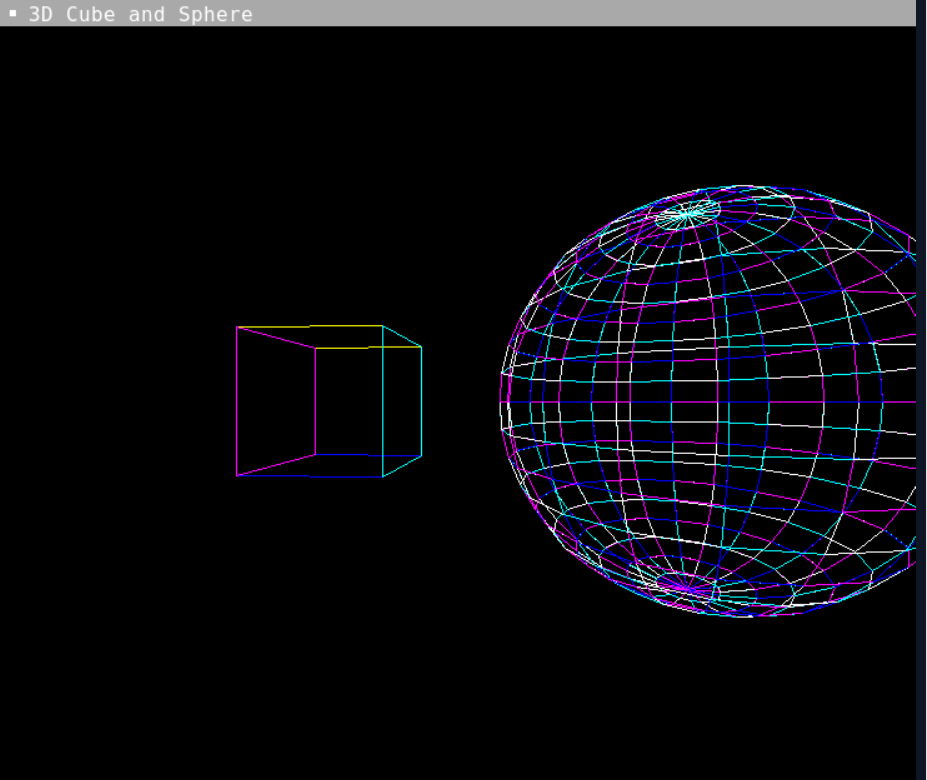
\includegraphics[width=0.5\textwidth]{1.png}
\end{center}

\textit{Exploration des Solutions et Choix Techniques}

\noindent Nous nous sommes d'abord tournés vers les fonctions classiques de SDL pour le remplissage de polygones, notamment \texttt{SDL\_RenderFillPolygon}. Cependant, nous nous sommes rapidement rendus compte que cette fonction n'était pas disponible ou non-fonctionnelle dans l'environnement de compilation que nous utilisions.

\textit{La Solution Retenue : \texttt{SDL\_RenderGeometryRaw}}

\noindent Après des recherches approfondies, nous avons découvert que la fonction \texttt{SDL\_RenderGeometryRaw} offrait une alternative plus appropriée pour le remplissage de polygones. Cette fonction, bien que plus complexe à utiliser, nous a permis de dessiner directement des polygones remplis. Son utilisation a nécessité une compréhension précise de la manière dont elle attend les données (notamment les sommets, les couleurs et les indices). L'utilisation de cette fonction a nécessité un certain temps d'adaptation et une bonne maitrise de ses paramètres.


\textit{Implications Techniques}

\noindent L'utilisation de \texttt{SDL\_RenderGeometryRaw} a eu plusieurs implications :
\begin{itemize}
\item Nous avons dû apprendre à manipuler des tableaux de données séparés pour les coordonnées des sommets et les couleurs, car cette fonction ne reçoit pas directement un tableau de structures \texttt{SDL\_Vertex}. Cela a nécessité un effort supplémentaire d'abstraction, car les coordonnées et les couleurs ne sont pas directement liées à un point en particulier.
   \item Nous avons aussi décidé de manipuler des tableaux de données plus élémentaires (des tableaux de \texttt{float} pour les coordonnées, des tableaux de \texttt{SDL\_Color} pour les couleurs, et un tableau d'entiers pour les indices), ce qui s'est avéré plus simple d'utilisation et plus performant.
\end{itemize}

\begin{center}
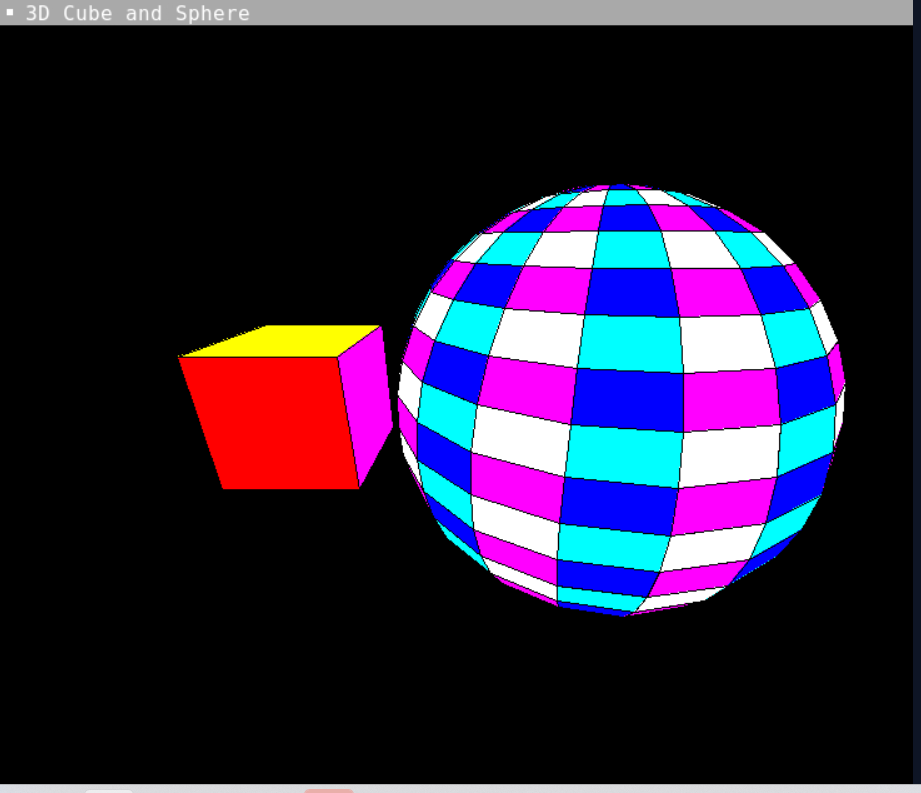
\includegraphics[width=0.5\textwidth]{3.png}
\end{center}

\subsection{Problèmes de Profondeur et Disparition des Faces}
\label{subsec:gestion_profondeur}

\textit{L'Apparition de Superpositions et de Disparitions Inattendues}

\noindent Nous avons rencontré des difficultés liées à la gestion de la profondeur des objets et à la visibilité des faces lors de la rotation. Plus précisément, les faces des objets les plus éloignés étaient parfois affichées par-dessus les faces plus proches, ce qui donnait un rendu incorrect de la profondeur. De plus, nous avons constaté que certaines faces disparaissaient lors des rotations des objets, causant un effet visuel perturbant. Cela suggérait des lacunes au niveau de la gestion de la visibilité des faces.

\begin{center}
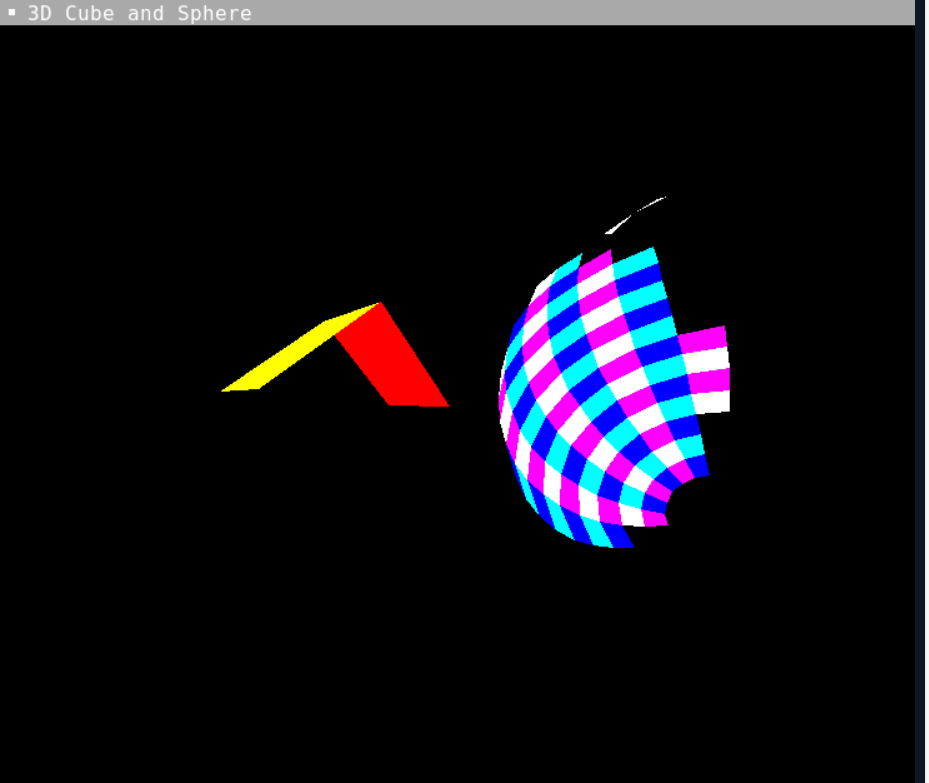
\includegraphics[width=0.5\textwidth]{2.png}
\end{center}

\noindent Nous avons d'abord cherché à comprendre comment gérer la visibilité des faces à l'aide d'un algorithme de "backface culling" que nous avons implémenté, qui consiste à ne pas afficher les faces qui étaient tournées vers l'arrière de la caméra, mais cette approche ne s'est pas avérée assez robuste et était la cause des disparitions. Nous avons aussi testé plusieurs approches du tri des polygones basées sur la profondeur, en tentant des implémentations différentes des algorithmes de tri, mais nous avons fini par utiliser \texttt{std::sort} qui était la plus performante.


\textit{La Solution Adoptée : Tri par Profondeur et Désactivation du Backface Culling}
\begin{itemize}
    \item \textbf{Implémentation du Tri par Profondeur} : Afin de gérer correctement l'ordre d'affichage, nous avons implémenté une méthode de tri par profondeur, dans laquelle les faces les plus éloignées de la caméra sont affichées avant les faces les plus proches. Cela a été rendu possible en utilisant une fonction \texttt{averageDepth()} qui calcule la moyenne de la coordonnée $z$ des sommets d'un quadrilatère, ce qui sert de critère pour trier les faces avec la fonction \texttt{std::sort}. L'utilisation de l'algorithme \textit{std::sort} de la bibliothèque standard a été le plus efficace et nous a permis de nous concentrer sur la logique du rendu plus que sur l'algorithme de tri lui même.
    \item \textbf{Désactivation du Backface Culling} : La méthode de "backface culling" que nous avions tentée d'implémenter (qui consiste à ne pas afficher les faces arrières) n'a pas fonctionné comme attendu et était à l'origine des disparitions de faces. Nous avons donc temporairement désactivé ce backface culling afin de stabiliser l'affichage et garantir que les objets soient visibles sous tous les angles. Bien que cette solution ne soit pas idéale (elle peut avoir un léger impact sur la performance et la visibilité), cela nous a permis de résoudre le problème de la disparition des faces pour l'instant.
\end{itemize}

\textit{Limitations et Pistes d'Amélioration}

\noindent Bien que ces solutions nous aient permis de corriger les problèmes de base, nous sommes conscients de leurs limites : la performance n'est pas optimale car nous trions toutes les faces à chaque rendu et nous affichons toutes les faces (au lieu de cacher les faces arrières), et la gestion de la profondeur reste une approche simplifiée. Il serait intéressant d'implémenter un vrai algorithme de Z-Buffer dans le futur pour améliorer l'affichage des objets.

\subsection{Organisation du Code et Gestion des Ressources SDL}
\label{subsec:gestion_ressources_sdl}

\textit{Difficulté Rencontrée : Problèmes d'Organisation et Gestion Inefficace des Ressources}

\noindent Au début de notre projet, l'initialisation et la gestion des ressources de la bibliothèque SDL (fenêtre, moteur de rendu) étaient dispersées directement dans la fonction \texttt{main()}. Cette approche présentait plusieurs inconvénients, tels qu'un code difficile à lire, à modifier et à maintenir, ainsi qu'un risque de fuites de mémoire.

\textit{Solution Adoptée : Création de la Classe \texttt{Sdl}}

\noindent Pour remédier à ces problèmes d'organisation, nous avons créé une classe nommée \texttt{Sdl} dédiée à la gestion des ressources de SDL. Cette classe encapsule l'initialisation de SDL (avec \texttt{SDL\_Init()}), la création de la fenêtre (avec \texttt{SDL\_CreateWindow()}) et du moteur de rendu (avec \texttt{SDL\_CreateRenderer()}), ainsi que la libération des ressources (avec \texttt{SDL\_DestroyRenderer()}, \texttt{SDL\_DestroyWindow()}, et \texttt{SDL\_Quit()}).

\textit{Avantages de l'Encapsulation}

\begin{itemize}
    \item  L'utilisation d'un constructeur permet de faire l'initialisation de SDL et la création de la fenêtre, du moteur de rendu en une seule ligne de code. On utilise une approche de \textit{RAII} (Resource Acquisition Is Initialization) dans le constructeur.
    \item  L'utilisation d'un destructeur permet de libérer les ressources SDL de manière automatique lors de la fin de l'exécution du programme. Cela a permis d'éviter les fuites de mémoire et de garantir un bon comportement du programme.
  \item L'encapsulation a permis d'avoir un code plus propre, plus modulaire, et a facilité sa maintenance et sa lecture.
\end{itemize}

\section{Conclusion}
\label{sec:conclusion}

\noindent Ce projet de développement d'un moteur 3D basique nous a apporté de précieuses connaissances et expériences dans le domaine de la programmation.

\subsection{Synthèse des Réalisations}

\noindent Nous avons réussi à concevoir une application qui :

\begin{itemize}
    \item Affiche des objets 3D (cube et sphère) sur un écran 2D.
    \item Applique des transformations de rotation et de translation de manière interactive et en temps réel.
    \item Utilise des couleurs distinctes pour chaque face des objets.
    \item Gère un tri par profondeur afin d'afficher les faces dans le bon ordre.
\end{itemize}

\subsection{Description de l'Interface et de son Utilisation}
\label{subsec:description_utilisation}

\noindent L'application que nous avons développée est interactive et permet de manipuler la scène 3D. Voici comment vous pouvez interagir avec notre moteur 3D \textbf{après avoir cliqué sur la fenêtre}:

\begin{itemize}
    \item \textbf{Rotations} : Les rotations autour des axes X et Y des objets sont contrôlées à l'aide des touches directionnelles du clavier (flèches).
    \item \textbf{Translations} : La translation (déplacement de toute la scène) est contrôlée à l'aide des touches \textit{W, A, S, D, Q et E} du clavier.
\end{itemize}
Il faut souligner que ces déplacements permettent d'interagir avec la scène en entier. L'affichage de l'écran se fait dans une fenêtre SDL, et l'application se termine en fermant la fenêtre.

\begin{center}
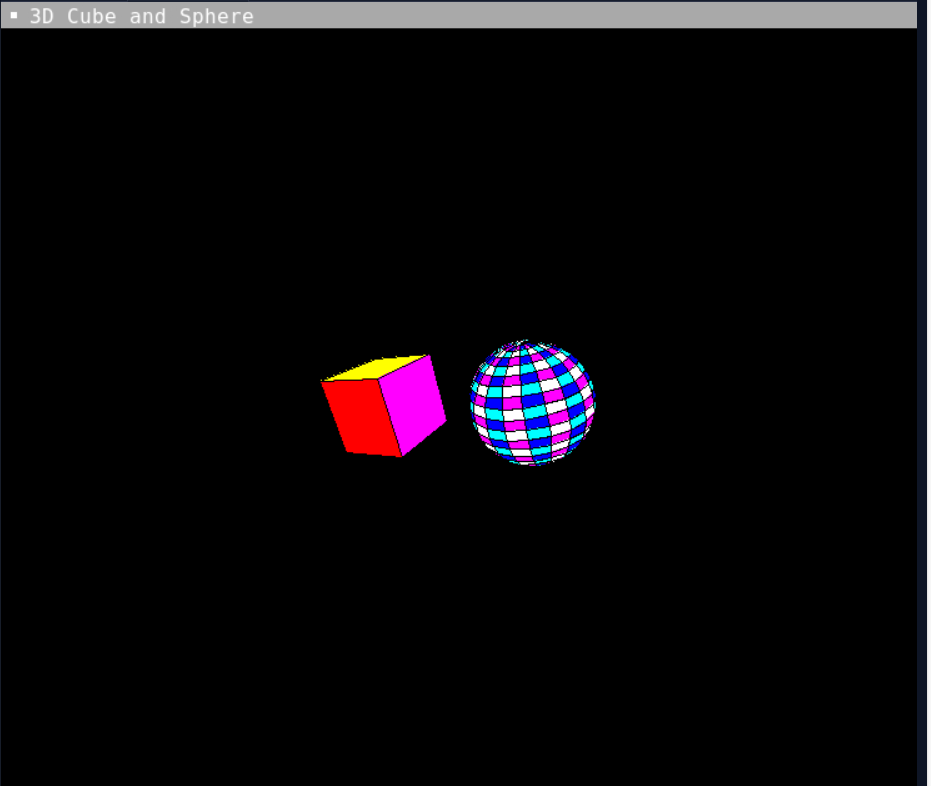
\includegraphics[width=0.5\textwidth]{4.png}
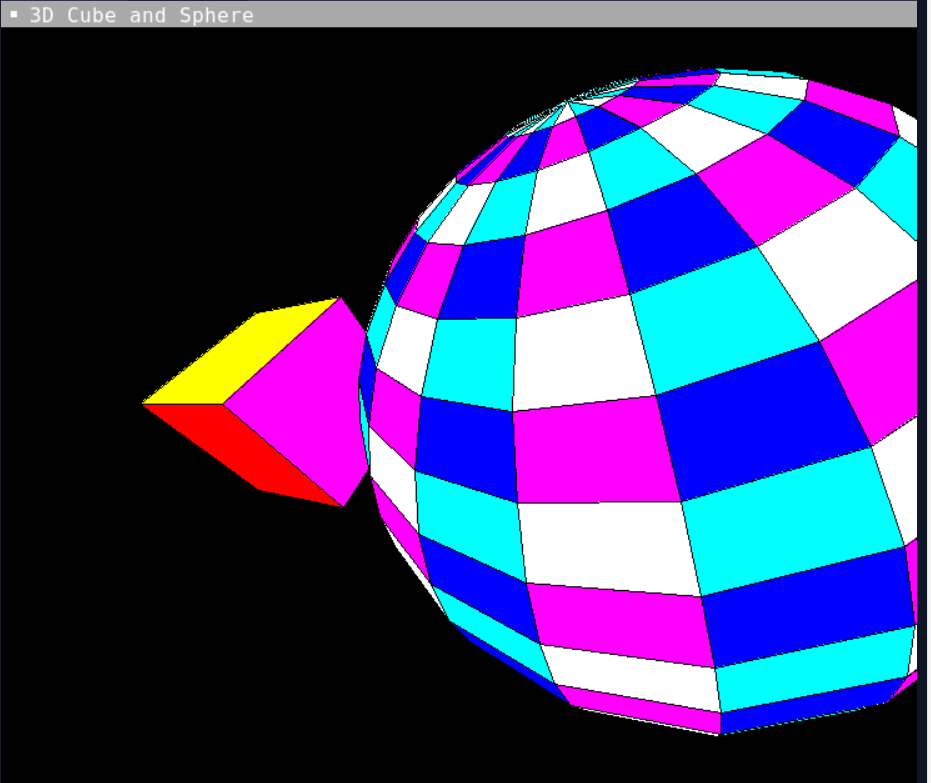
\includegraphics[width=0.5\textwidth]{5.png}
\end{center}

\subsection{Difficultés et Enseignements}

\noindent Ce projet nous a permis de mieux maîtriser le développement d'applications graphiques, et de développer nos compétences en programmation C++. Nous avons compris la complexité de certaines fonctions comme \texttt{SDL\_RenderGeometryRaw} qui sont très performantes mais qui nécessitent une bonne compréhension des mécanismes qu'elles utilisent. Les difficultés que nous avons rencontrées nous ont aidé à développer notre capacité de résolution de problèmes et à mieux maitriser les concepts fondamentaux du rendu 3D par rasterisation.

\subsection{Perspectives d'Avenir}
\label{subsec:perspectives_avenir}

\noindent Pour la suite, nous envisageons plusieurs améliorations afin de perfectionner notre moteur 3D :
\begin{itemize}
  \item \textbf{Implémentation de l'éclairage} : L'intégration de sources de lumière et de calculs d'éclairage pour rendre les objets plus réalistes.
  \item \textbf{Textures} : L'application de textures sur les objets afin d'améliorer leur aspect visuel.
    \item \textbf{Amélioration du Backface Culling} : Mettre en place une méthode robuste de Backface Culling afin d'éviter de dessiner les faces arrières et d'améliorer la performance du rendu.
    \item  \textbf{Implémentation d'un Z-Buffer} : Utiliser un Z-Buffer pour une gestion plus fine de la profondeur et améliorer la performance et le rendu des objets qui se chevauchent.
    \item \textbf{Ajout de formes géométriques} : Développer notre bibliothèque d'objets en ajoutant d'autres formes telles que des tores, des cônes, des cylindres, etc.
    \item \textbf{Optimisation de Performance} : Étudier les algorithmes de rendu et les optimiser pour améliorer la vitesse du moteur.
\end{itemize}



\end{document}